% chapitre de connexion et de création d'un compte
\chapter*{Se connecter à ou créer son compte}
\addcontentsline{toc}{chapter}{Se connecter à ou créer son compte}

La première chose à faire est de se connecter au site du portail qui est situé à \url{https://portail.apps.education.fr} comme le montre la capture d'écran suivante~:
\begin{figure}
    \centering
    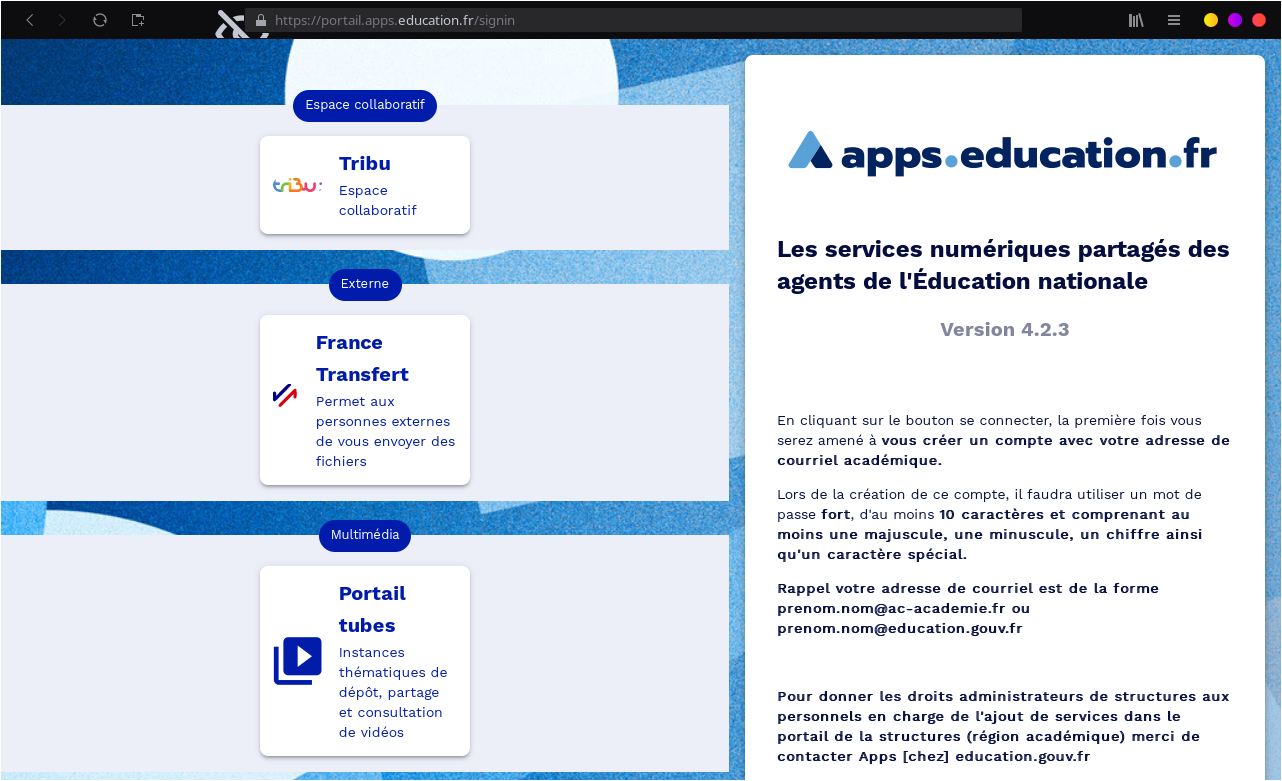
\includegraphics{Captures/portail.site.web.png}
\end{figure}

En bas à gauche se trouve le bouton \fbox{\hspace{1cm}SE~CONNECTER\hspace{1cm}} il donne alors accès à la fenêtre de connexion qui suit. 
\begin{figure}
	\centering
	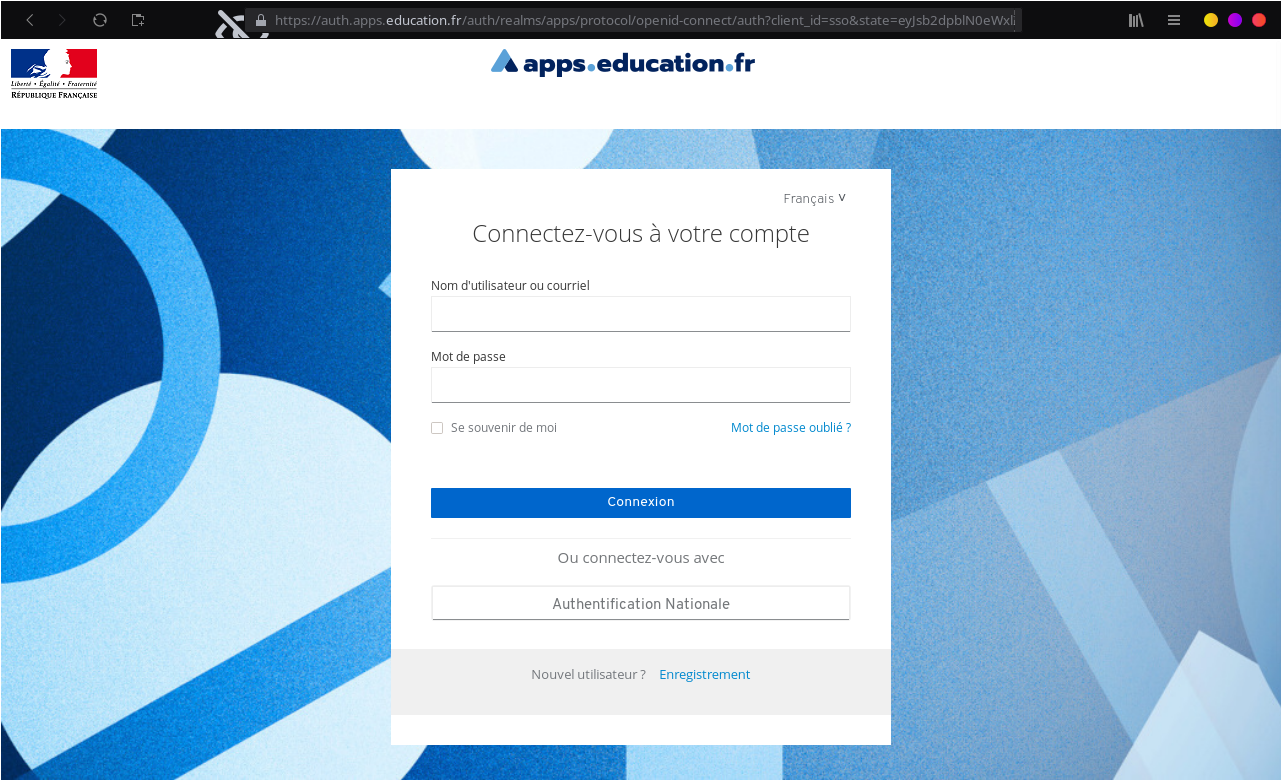
\includegraphics{./Captures/portail.site.web.connexion.png}
\end{figure}

Si on y regarde de plus près, on voit qu'on peut s'y connecter en saisissant son adresse professionnelle (académique ou ministérielle) mais également via un nom d'utilisateur. 
\begin{figure}
	\centering
	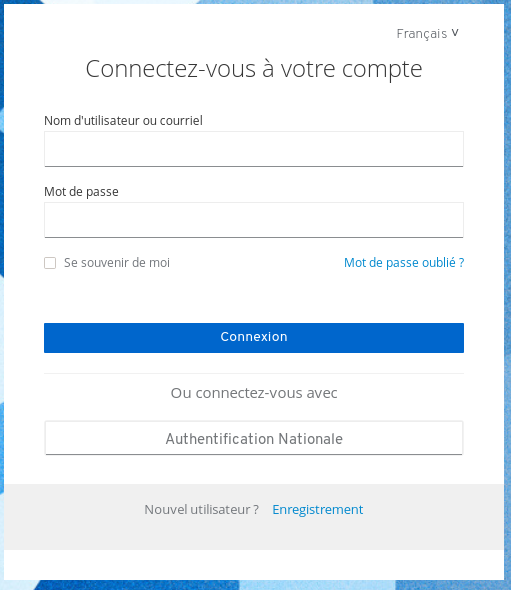
\includegraphics{./Captures/portail.site.web.connexion.zoom.png}
\end{figure}
Vers le bas de la fenêtre, une connexion avec ``Authentification Nationale'' est proposée, cette authentification sera abordée dans un \emph{attendum} ultérieur.

Évidemment la première fois impossible d'utiliser cette fenêtre de connxion puisque ``La Boîte'' ne nous connaît pas, aussi, la présence en bas à droite du lien \href{https://auth.apps.education.fr/auth/realms/apps/login-actions/registration?client_id=sso&tab_id=bVmOhc3T6kQ}{Enregistrement} va permettre l'inscription au service et à compter de ce moment-là cette fenêtre de connexion suffira.

La fenêtre d'enregistrement, comme cette capture, montre la présence en quatrième ligne d'un champ dédié à l'identifiant, c'est là qu'il faudra l'inventer en suivant les règles demandées et précisées en dessous du chmap.
\begin{figure}
	\centering
	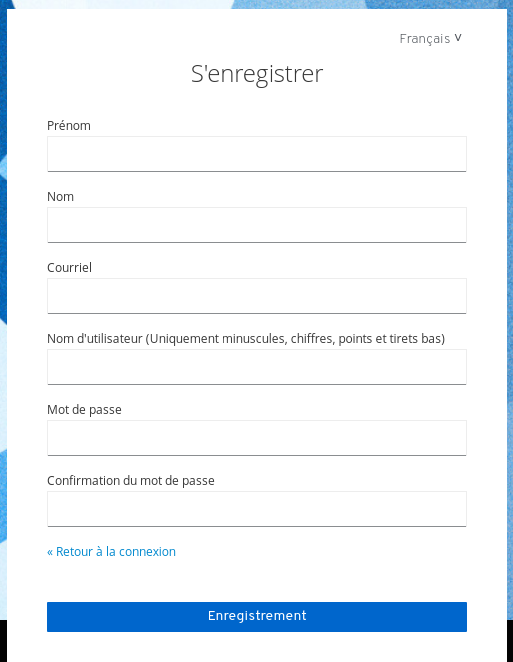
\includegraphics{./Captures/portail.site.web.enregistrement.png}
	\caption{}
\end{figure}

\paragraph{Avantage de l'identifiant.} Au cours d'une carrière nous sommes tous amenés à changer d'établissements, et une partie d'entre nous pour ne pas dire une majorité, nous changeons d'académie. 
Dès lors, le changement d'adresse mail s'opère pour chaque agent, et, comme l'intention de la boite est de rester un outil pérenne qui suit l'agent dans le temps, il faut pouvoir s'y connecter même en changeant de fonction ou d'académie, aussi la présence de cet identifiant vous permettra de vous connecter au compte et ensuite d'y modifier l'adressse mail de rattachement.

Une fois cette étape prête, un lien vers la fenêtre de connexion est visible si vous n'accédez pas directement au portail.
